\documentclass[[12pt,twoside]{book}
\usepackage{_my_document_style}
\begin{document}
%
\begin{myExampleX}{Zero lift angle of a cranked wing}{\ding{46}}% \ \Keyboard\ %
\label{example:Zero:Lift:Angle:Of:A:Cranked:Wing}
%
\def\mySpanWingMT{10.600000}
\def\mySpanWingIMT{6.360000}
\def\mySpanWingIIMT{4.240000}
\def\myChordRootWingMT{1.440000}
\def\myChordRootWingIMT{1.440000}
\def\myChordRootWingIIMT{1.440000}
\def\myChordTipWingMT{0.860000}
\def\myChordTipWingIMT{1.440000}
\def\myChordTipWingIIMT{0.860000}
\def\mySweepLEWingIIDEG{0.000000}
\def\myCoeffAChordWingI{0.000000}
\def\myCoeffBChordWingIMT{1.440000}
\def\myCoeffAChordWingII{-0.273585}
\def\myCoeffBChordWingIIMT{1.440000}
\def\myAlphaZeroLiftRootWingIDEG{-2.500000}
\def\myAlphaZeroLiftTipWingIDEG{-2.500000}
\def\myAlphaZeroLiftRootWingIRAD{-0.043633}
\def\myAlphaZeroLiftTipWingIRAD{-0.043633}
\def\myAlphaZeroLiftRootWingIIDEG{-2.500000}
\def\myAlphaZeroLiftTipWingIIDEG{-1.000000}
\def\myAlphaZeroLiftRootWingIIRAD{-0.043633}
\def\myAlphaZeroLiftTipWingIIRAD{-0.017453}
\def\myTaperRatioWingI{1.000000}
\def\myTaperRatioWingII{0.597222}
\def\myTwistWingIDEG{0.000000}
\def\myTwistWingIRAD{0.000000}
\def\myTwistWingIIDEG{-3.000000}
\def\myTwistWingIIRAD{-0.052360}
\def\myAreaWingIMTsquared{9.158400}
\def\myAreaWingIIMTsquared{4.876000}
\def\myAreaWingMTsquared{14.034400}
\def\myCoeffAAeroTwistWingIRADMT{0.000000}
\def\myCoeffBAeroTwistWingIRAD{-0.043633}
\def\myCoeffAAeroTwistWingIIRADMT{0.012349}
\def\myCoeffBAeroTwistWingIIRAD{-0.043633}
\def\myCoeffATwistWingIRADMT{0.000000}
\def\myCoeffATwistWingIIRADMT{-0.024698}
\def\myCoeffBTwistWingIRAD{0.000000}
\def\myCoeffBTwistWingIIRAD{0.000000}
\def\myAlphaZeroLiftWingIRAD{-0.028653}
\def\myAlphaZeroLiftWingIDEG{-1.641680}
\def\myAlphaZeroLiftWingIIRAD{0.008329}
\def\myAlphaZeroLiftWingIIDEG{0.477233}
\def\myAlphaZeroLiftWingRAD{-0.020323}
\def\myAlphaZeroLiftWingDEG{-1.164447}

%
%
\noindent
The right wing of a general aviation aircraft is shown in the figure~\ref{fig:Zero:Lift:Basic:1}. The planform has a straight leading edge and a straight piecewise trailing edge, with discontinuity in the point $B'$.
The wing is a special case of \emph{cranked wing} with
$\Lambda_\mathrm{le,1}=\Lambda_\mathrm{le,2}=\SI[round-precision=0]{\mySweepLEWingIIDEG}{\degree}$.
The total wingspan is $b=\SI[round-precision=1]{\mySpanWingMT}{\metre}$,the inner panel has extension $\frac{1}{2}b_1=\calcSI[round-precision=2,fixed-exponent=0,scientific-notation=fixed]{0.5*\mySpanWingIMT}{\metre}$,
the outer panel extension
$\frac{1}{2}b_2=\frac{1}{2}b-\frac{1}{2}b_1
=\calcSI[round-precision=2,fixed-exponent=0,scientific-notation=fixed]{0.5*\mySpanWingIIMT}{\metre}$.
The chord of the inner panel is constant and equal to
$c_\mathrm{r}=c_{\mathrm{r},1}=c_{\mathrm{t},1}=\SI[round-precision=2]{\myChordRootWingMT}{\metre}$.
The outer panel is instead tapered and has a tip chord
$c_\mathrm{t}=c_{\mathrm{t},2}=\SI[round-precision=2]{\myChordTipWingMT}{\metre}$.

Moreover, the inner panel has a constant profile and geometric twist.
Both at the root and at the tip of the first panel the zero lift angle of section is
$\alpha_{0\ell,\mathrm{r},1}=\alpha_{0\ell,\mathrm{t},1}=
\SI[round-precision=1]{\myAlphaZeroLiftRootWingIDEG}{\deg}$
and the geometric twist angle is
$\epsilon_{\mathrm{g,r},1}=\epsilon_{\mathrm{g,t},1}=\SI[round-precision=0]{\myTwistWingIDEG}{\deg}$.
In the outer panel there is a linear variation of the angle of zero lift and of the geometric twist angle;
the tip section has a zero lift angle
$\alpha_{0\ell,\mathrm{t},2}=\SI[round-precision=1]{\myAlphaZeroLiftTipWingIIDEG}{\deg}$.
and a geometric twist angle  
$\epsilon_{\mathrm{g,t},2}=\SI[round-precision=1]{\myTwistWingIIDEG}{\deg}$.
See the figure~\ref{fig:Zero:Lift:Cranked} for a graphical representation of the laws of $c(Y)$, $\alpha_{0\ell}(Y)$ and $\epsilon_\mathrm{g}(Y)$.

We want to calculate the zero lift angle of the wing: $\alpha_{0L}$.

\medskip
To solve the problem it is sufficient to reconstruct the analytical expressions of the laws of $c(Y)$, $\alpha_{0\ell}(Y)$ and $\epsilon_\mathrm{g}(Y)$
for $0\le Y \le \frac{1}{2}b$. Subsequently, these piecewise linear laws must be replaced in the definite integral which is in the calculation formula of $\alpha_{0L}$.

The chord law of the given planform is the following piecewise linear function:
\[
c(Y)=
\begin{cases}
%\left\{
%\begin{array}{cl}
c_1(Y) = A_{c,1} \, Y + B_{c,1} & \text{per }\makebox[3em][r]{$0$}     \le Y \le \frac{1}{2}b_1
\\[4pt]
c_2(Y) = A_{c,2} \, \bigg(Y-\dfrac{b_1}{2}\bigg) + B_{c,2} & \text{per }\makebox[3em][r]{$\frac{1}{2}b_1$}< Y \le \frac{1}{2}b
%\end{array}
%\right.
\end{cases}
\]
whose coefficients are calculated by imposing $c_1(0)=c_{\mathrm{r},1}$,
$c_1(\frac{1}{2}b_1)=c_{\mathrm{t},1}$, $c_2(\frac{1}{2}b_1)=c_{\mathrm{r},2}$, $c_2(\frac{1}{2}b)=c_{\mathrm{t},2}$.
For assigned data we have
\[
A_{c,1}
  = \frac{c_{\mathrm{t},1} - c_{\mathrm{r},1}}{b_1/2}
  = 
    2 \frac{
      \SI[round-precision=2]{\myChordTipWingIMT}{\metre} - \SI[round-precision=2]{\myChordRootWingIMT}{\metre}
    }{
      \SI[round-precision=2]{\mySpanWingIMT}{\metre}
    }
  = \mathunderline{mydarkblue}{ \SI[round-precision=0]{\myCoeffAChordWingI}{} }
\]
\[
B_{c,1}
  = c_{\mathrm{r},1}
  = \mathunderline{mydarkblue}{ \SI[round-precision=2]{\myCoeffBChordWingIMT}{\metre} }
\]
\[
A_{c,2}
  = \frac{c_{\mathrm{t},2} - c_{\mathrm{r},2}}{b_2/2}
  = 
    2 \frac{
      \SI[round-precision=2]{\myChordTipWingIIMT}{\metre} - \SI[round-precision=2]{\myChordRootWingIIMT}{\metre}
    }{
      \SI[round-precision=2]{\mySpanWingIIMT}{\metre}
    }
  = \mathunderline{mydarkblue}{ \SI[round-precision=3]{\myCoeffAChordWingII}{} }
\]
\[
B_{c,2}
  = c_{\mathrm{r},2}
  = \mathunderline{mydarkblue}{ \SI[round-precision=2]{\myCoeffBChordWingIIMT}{\metre} }
\]
therefore
\[
c(Y)=
\begin{cases}
%\left\{
%\begin{array}{cl}
c_1(Y) = 
  %% ZERO -> \SI[round-precision=3]{\myCoeffAChordWingI}{} \, Y 
    % + 
    \SI[round-precision=2]{\myCoeffBChordWingIIMT}{\metre} 
  & \text{per }
    \makebox[3.5em][r]{$\SI[round-precision=0]{0}{\metre}$} 
      \le Y \le 
      \calcSI[round-precision=2,fixed-exponent=0,scientific-notation=fixed]{0.5*\mySpanWingIMT}{\metre}
\\[4pt]
c_2(Y) 
  = \SI[round-precision=3]{\myCoeffAChordWingII}{} \, 
    \big(
      Y
      - \calcSI[round-precision=2,fixed-exponent=0,scientific-notation=fixed]{0.5*\mySpanWingIMT}{\metre}
    \big)
    + \SI[round-precision=2]{\myCoeffBChordWingIIMT}{\metre} 
  & \text{per }
    \makebox[3.5em][r]{%
      $\calcSI[round-precision=2,fixed-exponent=0,scientific-notation=fixed]{0.5*\mySpanWingIMT}{\metre}$
    }% end-of-makebox
      < Y 
      \le \calcSI[round-precision=2,fixed-exponent=0,scientific-notation=fixed]{0.5*\mySpanWingMT}{\metre}
%\end{array}
%\right.
\end{cases}
\]

The law of section zero lift angles is the following piecewise linear function:
\[
\alpha_{0\ell}(Y)=
\begin{cases}
%\left\{
%\begin{array}{cl}
\alpha_{0\ell,1}(Y) = A_{\alpha,1} \, Y + B_{\alpha,1} & \text{per }\makebox[3em][r]{$0$}     \le Y \le \frac{1}{2}b_1
\\[4pt]
\alpha_{0\ell,2}(Y) = A_{\alpha,2} \, \bigg(Y-\dfrac{b_1}{2}\bigg) + B_{\alpha,2} & \text{per }\makebox[3em][r]{$\frac{1}{2}b_1$}< Y \le \frac{1}{2}b
%\end{array}
%\right.
\end{cases}
\]
whose coefficients are calculated by imposing $\alpha_{0\ell,1}(0)=\alpha_{0\ell,\mathrm{r},1}$,
$\alpha_{0\ell,1}(\frac{1}{2}b_1)=\alpha_{0\ell,\mathrm{t},1}$, $\alpha_{0\ell,2}(\frac{1}{2}b_1)=\alpha_{0\ell,\mathrm{r},2}$, $\alpha_{0\ell,2}(\frac{1}{2}b)=\alpha_{0\ell,\mathrm{t},2}$.
For assigned data we have
\[
A_{\alpha,1}
  = \frac{\alpha_{0\ell,\mathrm{t},1} - \alpha_{0\ell,\mathrm{r},1}}{b_1/2}
  = 
    2 \frac{
      \SI[round-precision=2]{\myAlphaZeroLiftTipWingIRAD}{\radian} - ( \SI[round-precision=2]{\myAlphaZeroLiftRootWingIRAD}{\radian} )
    }{
      \SI[round-precision=2]{\mySpanWingIMT}{\metre}
    }
  = \mathunderline{mydarkblue}{ \SI[round-precision=0]{\myCoeffAAeroTwistWingIRADMT}{\radian/\metre} }
\]
\[
B_{\alpha,1}
  = \alpha_{0\ell,\mathrm{r},1}
  = \mathunderline{mydarkblue}{ \SI[round-precision=4]{\myCoeffBAeroTwistWingIRAD}{\radian} }
\]
\[
A_{\alpha,2}
  = \frac{\alpha_{0\ell,\mathrm{t},2} - \alpha_{0\ell,\mathrm{r},2}}{b_2/2}
  = 
    2 \frac{
      \SI[round-precision=4]{\myAlphaZeroLiftTipWingIIRAD}{\metre} - ( \SI[round-precision=4]{\myAlphaZeroLiftRootWingIIRAD}{\metre} )
    }{
      \SI[round-precision=2]{\mySpanWingIIMT}{\metre}
    }
  = \mathunderline{mydarkblue}{ \SI[round-precision=4]{\myCoeffAAeroTwistWingIIRADMT}{\radian/\metre} }
\]
\[
B_{\alpha,2}
  = \alpha_{0\ell,\mathrm{r},2}
  = \mathunderline{mydarkblue}{ \SI[round-precision=4]{\myCoeffBAeroTwistWingIIRAD}{\radian} }
\]
So
\[
\alpha_{0\ell}(Y)=
\begin{cases}
%\left\{
%\begin{array}{cl}
\alpha_{0\ell,1}(Y) = 
  %% ZERO -> \SI[round-precision=3]{\myCoeffAAeroTwistWingIRADMT}{\radian/\metre} \, Y 
    % + 
    \SI[round-precision=0]{\myCoeffBAeroTwistWingIRAD}{\radian} 
  & \text{per }
    \makebox[3.5em][r]{$\SI[round-precision=0]{0}{\metre}$} 
      \le Y \le 
      \calcSI[round-precision=2,fixed-exponent=0,scientific-notation=fixed]{0.5*\mySpanWingIMT}{\metre}
\\[4pt]
\alpha_{0\ell,2}(Y) 
  = \SI[round-precision=4]{\myCoeffAAeroTwistWingIIRADMT}{\radian/\metre} \; 
    \big(
      Y
      - \calcSI[round-precision=2,fixed-exponent=0,scientific-notation=fixed]{0.5*\mySpanWingIMT}{\metre}
    \big)
   %% + \SI[round-precision=4]{\myCoeffBAeroTwistWingIIRAD}{\radian} 
   \rule{2em}{0pt}% --> SPACER
%
\\
    \hfill
    \SI[round-precision=0]{\myCoeffBAeroTwistWingIIRAD}{\radian}
%
  & \text{per }
    \makebox[3.5em][r]{%
      $\calcSI[round-precision=2,fixed-exponent=0,scientific-notation=fixed]{0.5*\mySpanWingIMT}{\metre}$
    }% end-of-makebox
      < Y 
      \le \calcSI[round-precision=2,fixed-exponent=0,scientific-notation=fixed]{0.5*\mySpanWingMT}{\metre}
%\end{array}
%\right.
\end{cases}
\]

Finally, the law of geometric section twist angles is the following piecewise linear function:
\[
\epsilon_{\mathrm{g}}(Y)=
\begin{cases}
%\left\{
%\begin{array}{cl}
\epsilon_{\mathrm{g},1}(Y) = A_{\epsilon,1} \, Y + B_{\epsilon,1} & \text{per }\makebox[3em][r]{$0$}     \le Y \le \frac{1}{2}b_1
\\[4pt]
\epsilon_{\mathrm{g},2}(Y) = A_{\epsilon,2} \, \bigg(Y-\dfrac{b_1}{2}\bigg) + B_{\epsilon,2} & \text{per }\makebox[3em][r]{$\frac{1}{2}b_1$}< Y \le \frac{1}{2}b
%\end{array}
%\right.
\end{cases}
\]
whose coefficients are calculated by imposing $\epsilon_{\mathrm{g},1}(0)=\SI[round-precision=0]{0}{\deg}$,
$\epsilon_{\mathrm{g},1}(\frac{1}{2}b_1)=\epsilon_{\mathrm{g,t},1}$, $\epsilon_{\mathrm{g},2}(\frac{1}{2}b_1)=\epsilon_{\mathrm{g,t},1}$, $\epsilon_{\mathrm{g},2}(\frac{1}{2}b)=\epsilon_{\mathrm{g,t},2}$.
For assigned data we have
\[
A_{\epsilon,1}
  = \frac{\epsilon_{\mathrm{g,t},1}}{b_1/2}
  = 
    2 \frac{
      \SI[round-precision=2]{\myTwistWingIRAD}{\radian}
    }{
      \SI[round-precision=2]{\mySpanWingIMT}{\metre}
    }
  = \mathunderline{mydarkblue}{ \SI[round-precision=0]{\myCoeffATwistWingIRADMT}{\radian/\metre} }
\]
\[
B_{\epsilon,1}
  = \epsilon_{\mathrm{g,r},1}
  = \mathunderline{mydarkblue}{ \SI[round-precision=0]{\myCoeffBTwistWingIRAD}{\radian} }
\]
\[
A_{\epsilon,2}
  = \frac{\epsilon_{\mathrm{g,t},2} - \epsilon_{\mathrm{g,r},2}}{b_2/2}
  = 
    2 \frac{
      \SI[round-precision=4]{\myTwistWingIIRAD}{\metre} - ( \SI[round-precision=4]{\myTwistWingIRAD}{\metre} )
    }{
      \SI[round-precision=2]{\mySpanWingIIMT}{\metre}
    }
  = \mathunderline{mydarkblue}{ \SI[round-precision=4]{\myCoeffATwistWingIIRADMT}{\radian/\metre} }
\]
\[
B_{\epsilon,2}
  = \epsilon_{\mathrm{g,r},2}
  = \mathunderline{mydarkblue}{ \SI[round-precision=0]{\myCoeffBTwistWingIIRAD}{\radian} }
\]
therefore
\[
\epsilon_{\mathrm{g}}(Y)=
\begin{cases}
%\left\{
%\begin{array}{cl}
\epsilon_{\mathrm{g},1}(Y) = 
  %% ZERO -> \SI[round-precision=3]{\myCoeffAAeroTwistWingIRADMT}{\radian/\metre} \, Y 
    % + 
    \SI[round-precision=0]{\myCoeffBTwistWingIRAD}{\radian} 
  & \text{per }
    \makebox[3.5em][r]{$\SI[round-precision=0]{0}{\metre}$} 
      \le Y \le 
      \calcSI[round-precision=2,fixed-exponent=0,scientific-notation=fixed]{0.5*\mySpanWingIMT}{\metre}
\\[4pt]
\epsilon_{\mathrm{g},2}(Y) 
  = \SI[round-precision=4]{\myCoeffATwistWingIIRADMT}{\radian/\metre} \; 
    \big(
      Y
      - \calcSI[round-precision=2,fixed-exponent=0,scientific-notation=fixed]{0.5*\mySpanWingIMT}{\metre}
    \big)
   %% + \SI[round-precision=4]{\myCoeffBAeroTwistWingIIRAD}{\radian} 
%   \rule{2em}{0pt}% --> SPACER
%
% \\
%    \hfill
%    \SI[round-precision=4]{\myCoeffBTwistWingIIRAD}{\radian}
%
  & \text{per }
    \makebox[3.5em][r]{%
      $\calcSI[round-precision=2,fixed-exponent=0,scientific-notation=fixed]{0.5*\mySpanWingIMT}{\metre}$
    }% end-of-makebox
      < Y 
      \le \calcSI[round-precision=2,fixed-exponent=0,scientific-notation=fixed]{0.5*\mySpanWingMT}{\metre}
%\end{array}
%\right.
\end{cases}
\]
At this point it's possible to calculate the angle of zero lift
\[
\alpha_{0L} 
  = \frac{2}{S} \int_0^{b/2} 
    \Big[ 
      \alpha_{0\ell}\big(Y\big) - \epsilon_\mathrm{g}\big(Y\big) 
    \Big] \, c(Y) \diff{Y}
\]
that for a \emph{cranked} wing with two panels becomes a sum of two integrals
\[
\begin{split}
\alpha_{0L} 
  & {}= 
    \frac{2}{S} \int_0^{b_1/2} 
    \Big[ 
      \alpha_{0\ell,1}\big(Y\big) - \epsilon_{\mathrm{g},1}\big(Y\big) 
    \Big] \, c_1(Y) \diff{Y}
\\[3pt]
  &
  \rule{0.25\linewidth}{0pt}% --> SPACER
  +
    \frac{2}{S} \int_{b_1/2}^{b/2}
    \Big[ 
      \alpha_{0\ell,2}\big(Y\big) - \epsilon_{\mathrm{g},2}\big(Y\big) 
    \Big] \, c_2(Y) \diff{Y}
\end{split}
\]
The previous formula, written in full, becomes
\[
\begin{split}
\alpha_{0L} 
  & {}= \frac{2}{S} \int_0^{b_1/2} 
    \bigg[ \Big( A_{\alpha,1} \, Y + B_{\alpha,1} \Big) - A_{\epsilon,1} \, Y \bigg] \Big( A_{c,1} Y + B_{c,1} \Big)
      \diff{Y} \hfill \mbox{}
\\[3pt]
  &  
    \rule{3em}{0pt}% --> SPACER
    %\mbox{} \hfill 
    + \frac{2}{S} \int_{b_1/2}^{b/2} 
    \bigg[ A_{\alpha,2} \, \Big( Y - \frac{b_1}{2} \Big) + B_{\alpha,2} 
      - A_{\epsilon,2} \, \Big( Y - \frac{b_1}{2} \Big) - B_{\epsilon,2}\bigg] 
   \rule{1em}{0pt}% --> SPACER
\\[3pt]
  &  
    \rule{22em}{0pt}% --> SPACER
    \cdot \bigg[ A_{c,2} \Big( Y - \frac{b_1}{2} \Big) + B_{c,2} \bigg]
      \diff{Y}
\end{split}
\]

The panels of the assigned wing have a taper ratio:
\[
\lambda_1
  =\frac{c_{\mathrm{t},1}}{c_{\mathrm{r},1}}
  =\frac{\SI[round-precision=2]{\myChordTipWingIMT}{\metre}}{\SI[round-precision=2]{\myChordRootWingIMT}{\metre}}
  =\mathunderline{mydarkblue}{ \SI[round-precision=0]{\myTaperRatioWingI}{} }
\]
\[
\lambda_2
  =\frac{c_{\mathrm{t},2}}{c_{\mathrm{r},2}}
  =\frac{\SI[round-precision=2]{\myChordTipWingIIMT}{\metre}}{\SI[round-precision=2]{\myChordRootWingIIMT}{\metre}}
  =\mathunderline{mydarkblue}{ \SI[round-precision=2]{\myTaperRatioWingII}{} }
\]
and surfaces 
\[
\begin{split}
S_1 & {}= \frac{b_1}{2} \, c_{\mathrm{r},1} \, \big( 1 + \lambda_1 \big) \\
  & {}=
    \num{0.5} \cdot \SI[round-precision=1]{\mySpanWingIMT}{\metre}
      \cdot \SI[round-precision=2]{\myChordRootWingIMT}{\metre}
      \cdot \big( 1 + \SI[round-precision=2]{\myTaperRatioWingI}{} \big) 
    = \mathunderline{mydarkblue}{ \SI[round-precision=2]{\myAreaWingIMTsquared}{\metre^2} }
\end{split}
\]
\[
\begin{split}
S_2 & {}= \frac{b_2}{2} \, c_{\mathrm{r},2} \, \big( 1 + \lambda_2 \big) \\
  & {}=
    \num{0.5} \cdot \SI[round-precision=1]{\mySpanWingIIMT}{\metre}
      \cdot \SI[round-precision=2]{\myChordRootWingIIMT}{\metre}
      \cdot \big( 1 + \SI[round-precision=2]{\myTaperRatioWingII}{} \big) 
    = \mathunderline{mydarkblue}{ \SI[round-precision=2]{\myAreaWingIIMTsquared}{\metre^2} }
\end{split}
\]
Therefore, the wing area is
\[
\begin{split}
S = S_1 + S_2 
  = \SI[round-precision=2]{\myAreaWingIMTsquared}{\metre^2}
    + \SI[round-precision=2]{\myAreaWingIIMTsquared}{\metre^2}
  = \mathunderline{mydarkblue}{ \SI[round-precision=2]{\myAreaWingMTsquared}{\metre^2} }
\end{split}
\]

The sum of the two definite integrals is easily obtained by substituting the values in the integrating functions
of the previously calculated coefficients.
Carrying out the calculations for the first integral we obtain
\[
\begin{split}
\alpha_{0L,1} 
  & {}= \frac{2}{S} \int_0^{b_1/2} 
    \bigg[ \Big( A_{\alpha,1} \, Y + B_{\alpha,1} \Big) - A_{\epsilon,1} \, Y \bigg] \Big( A_{c,1} Y + B_{c,1} \Big)
      \diff{Y} \hfill \mbox{}
\\[3pt]
   & ={}
     \frac{2}{ \SI[round-precision=2]{\myAreaWingMTsquared}{\metre^2} }
     \int_{\SI{0}{m}}^{
       \calcSI[round-precision=1,fixed-exponent=0,scientific-notation=fixed]{0.5*\mySpanWingIMT}{\metre}
     }
     \Big[ 
       \Big( 
         % A_{\alpha} \, Y + B_{\alpha} 
         \SI[round-precision=0]{\myCoeffAAeroTwistWingIRADMT}{\radian/\metre} \; Y
           \SI[round-precision=4]{\myAlphaZeroLiftRootWingIRAD}{\radian}
       \Big) 
\\
  & \rule{0.3\linewidth}{0pt}% --> SPACER
       % - A_{\epsilon} \, Y 
       - ( \SI[round-precision=0]{\myCoeffATwistWingIRADMT}{\radian/\metre} ) \; Y
     \Big] 
     \Big( 
       \SI[round-precision=0]{\myCoeffAChordWingI}{} \; Y
         + \SI[round-precision=2]{\myCoeffBChordWingIMT}{\metre}
       \Big) \diff{Y}
\\
   & ={}
     \frac{2}{ \SI[round-precision=2]{\myAreaWingMTsquared}{\metre^2} }
     \int_{\SI{0}{m}}^{
       \calcSI[round-precision=1,fixed-exponent=0,scientific-notation=fixed]{0.5*\mySpanWingIMT}{\metre}
     }
           \SI[round-precision=4]{\myAlphaZeroLiftRootWingIRAD}{\radian}
         \cdot \SI[round-precision=2]{\myCoeffBChordWingIMT}{\metre}
       \diff{Y}
\\[2pt]
  & {}= \mathunderline{mydarkblue}{ \SI[round-precision=4]{\myAlphaZeroLiftWingIRAD}{\radian} }
  = \mathunderline{mydarkblue}{ \SI[round-precision=2]{\myAlphaZeroLiftWingIDEG}{\deg} }
\end{split}
\]

Similarly, for the second integral we obtain
\[
\begin{split}
\alpha_{0L,2} 
  & {}= \frac{2}{S} \int_{b_1/2}^{b/2} 
    \bigg[ A_{\alpha,2} \, \Big( Y - \frac{b_1}{2} \Big) + B_{\alpha,2} 
      - A_{\epsilon,2} \, \Big( Y - \frac{b_1}{2} \Big) - B_{\epsilon,2}\bigg] 
   \rule{1em}{0pt}% --> SPACER
\\[3pt]
  &  
    \rule{22em}{0pt}% --> SPACER
    \cdot \bigg[ A_{c,2} \Big( Y - \frac{b_1}{2} \Big) + B_{c,2} \bigg]
      \diff{Y}
\\
  & ={}
    \frac{2}{ \SI[round-precision=1]{\myAreaWingMTsquared}{\metre^2} }
    \int_{
      \calcSI[round-precision=1,fixed-exponent=0,scientific-notation=fixed]{0.5*\mySpanWingIMT}{\metre}
    }^{
      \calcSI[round-precision=1,fixed-exponent=0,scientific-notation=fixed]{0.5*\mySpanWingMT}{\metre}
    }
    \Big[ 
      % A_{\alpha} \, Y + B_{\alpha} 
      \SI[round-precision=4]{\myCoeffAAeroTwistWingIIRADMT}{\radian/\metre} \; \Big( Y
        - \calcSI[round-precision=1,fixed-exponent=0,scientific-notation=fixed]{0.5*\mySpanWingIMT}{\metre} \Big)
        \SI[round-precision=4]{\myAlphaZeroLiftRootWingIIRAD}{\radian}
\\
  & \rule{0.3\linewidth}{0pt}% --> SPACER
       % - A_{\epsilon} \, Y 
       - ( \SI[round-precision=4]{\myCoeffATwistWingIIRADMT}{\radian/\metre} ) \; \Big( Y
           - \calcSI[round-precision=1,fixed-exponent=0,scientific-notation=fixed]{0.5*\mySpanWingIMT}{\metre} \Big)
           - \SI[round-precision=2]{\myCoeffBTwistWingIIRAD}{\radian}
     \Big]
\\
  & \rule{0.5\linewidth}{0pt}% --> SPACER
     \Big[ 
       \SI[round-precision=3]{\myCoeffAChordWingII}{} \; \Big( Y
           - \calcSI[round-precision=1,fixed-exponent=0,scientific-notation=fixed]{0.5*\mySpanWingIMT}{\metre} \Big)
         + \SI[round-precision=2]{\myCoeffBChordWingIIMT}{\metre}
       \Big] \diff{Y}
\\[2pt]
  & {}= \mathunderline{mydarkblue}{ \SI[round-precision=5]{\myAlphaZeroLiftWingIIRAD}{\radian} }
  = \mathunderline{mydarkblue}{ \SI[round-precision=2]{\myAlphaZeroLiftWingIIDEG}{\deg} }
\end{split}
\]

Finally, the zero lift angle of the assigned wing is
\[
\begin{split}
\alpha_{0L} = \alpha_{0L,1} + \alpha_{0L,2} 
  & {}= \SI[round-precision=4]{\myAlphaZeroLiftWingIRAD}{\radian}
    + ( \SI[round-precision=5]{\myAlphaZeroLiftWingIIRAD}{\radian} )
\\
  & {}= \mathunderline{mydarkblue}{ \SI[round-precision=4]{\myAlphaZeroLiftWingRAD}{\radian} }
    = \mathunderline{mydarkblue}{ \SI[round-precision=2]{\myAlphaZeroLiftWingDEG}{\deg} }
\end{split}
\]
%
\begin{figure}[t]%[H]%[!htbp]
  \centering
  %\checkoddpage
  %\centering
    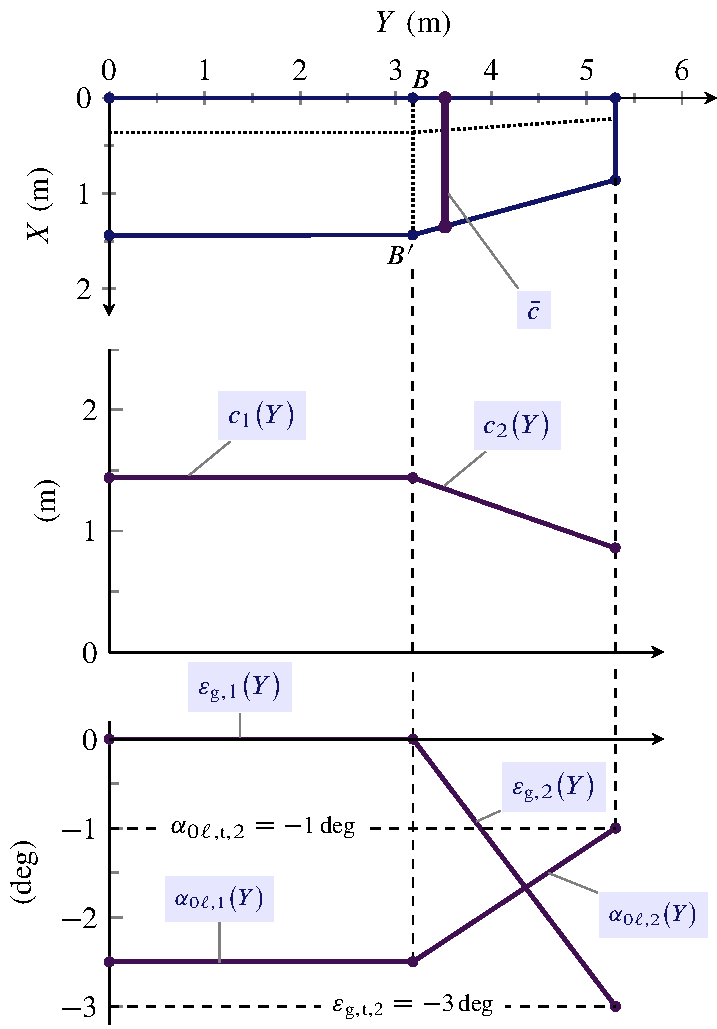
\includegraphics[width=0.78\textwidth]{Chapter_2/zero_lift_angle_of_a_cranked_wing/wing_alpha_zero_lift_1A_drawing.pdf}
  \caption{\finalhyphendemerits=1000
           Planform of the cranked wing assigned in the example~\ref{example:Zero:Lift:Angle:Of:A:Cranked:Wing}.The linear laws of the chords, of the zero lift angle of section and geometric twist angle are also reported
 }
  \label{fig:Zero:Lift:Cranked}%
\end{figure}
%
\end{myExampleX}
\end{document}